\documentclass[%
 reprint,
 amsmath,amssymb,
 aps,
 prb,
]{revtex4-2}

% Basic packages
\usepackage{graphicx}
\usepackage{bm}
\usepackage{physics}
\usepackage[colorlinks=true,
            linkcolor=blue,
            filecolor=blue,
            urlcolor=blue,
            citecolor=blue]{hyperref}
\usepackage{caption}
\captionsetup[figure]{justification=justified,labelfont={bf},name={Fig.},labelsep=period}
\captionsetup[table]{justification=justified,labelfont={bf},name={Table},labelsep=period}
\numberwithin{equation}{section}
\usepackage[final]{microtype}
\usepackage{ragged2e}
\usepackage{booktabs}

% Add the following packages to the existing preamble
\usepackage{amsmath}
\usepackage{tikz}
\usetikzlibrary{arrows.meta, calc, 3d, shadings, positioning}

\newtheorem{theorem}{Theorem}[section]
\newcommand{\iphase}{\theta}

\begin{document}

\title{Geometrical Confinement of Energy in the 0-Sphere Model:
\\A Topological Mechanism Underlying Rest Mass and Zitterbewegung}

\author{Satoshi Hanamura}
\email{hana.tensor@gmail.com}
\date{January 24, 2026}

\begin{abstract}
We present a geometrical interpretation of the 0-Sphere model in which thermal potential energy—identified with rest mass energy—is localized at two discrete energy kernels, while admissible radiative transport is constrained by an embedding into a higher-dimensional arcwise connected region interpreted as a photon sphere.
Although the 0-sphere itself is totally disconnected, its embedding into this compact domain permits continuous paths that support circulation of thermal potential energy between kernels via Zitterbewegung oscillations derived from the Dirac equation.
This construction establishes a topological mechanism in which rest mass and Zitterbewegung emerge from geometric confinement rather than from dynamical binding or symmetry-based conservation laws.
The resulting confinement is topological rather than dynamical, restricting radiative processes to a finite region and ensuring energy conservation without invoking dynamical equations of motion or Noether-type symmetries.
The framework clarifies the coexistence of discrete localization and continuous transport, and provides a controlled description of extreme limits in which admissible transport structures degenerate.
\end{abstract}


\maketitle

% ========================================
% Section 1: Introduction
% ========================================
\section{Introduction}
\label{sec:introduction}

The 0-Sphere model characterizes physical degrees of freedom using the simplest nontrivial topological structure: a pair of isolated points forming a 0-sphere.
In this framework, the two points correspond to discrete energy kernels (kernel $A$ and kernel $B$) whose thermal potential energy represents localized configurations capable of oscillatory exchange.
Despite its minimalism, the model has been argued to encode essential aspects of localized energy kernels and their associated behavior.
A persistent source of ambiguity, however, concerns how such a totally disconnected structure may accommodate physically meaningful notions of transport, circulation, or radiation between these kernels.

In the present work~\cite{hanamura18067760,hanamura18135855,hanamura18203433}, this ambiguity is resolved by separating, at a structural level, discrete localization from continuous transport.
We emphasize that no continuous path exists within the 0-sphere itself, and that any admissible transport must therefore be associated with an embedding into a higher-dimensional region that supplies the necessary arcwise connectivity.

Within the physical interpretation of the 0-Sphere model, the two points correspond to discrete internal energy kernels (denoted kernel $A$ and kernel $B$ in earlier work), between which thermal potential energy—identified with rest mass energy—circulates through alternating phases of radiation and absorption.
When the system resides entirely at kernel $A$ (corresponding to complete temporal phase localization), the full rest mass energy must be radiated in order to achieve transfer to kernel $B$.
The embedding region $\mathcal{D}$ is interpreted as a \textit{photon sphere}: a spatially confined domain containing both kernels and supporting internal radiative circulation.
Admissible radiative paths within $\mathcal{D}$ are not arbitrary but follow geodesics determined by a least-action principle, analogous to Snell-type refraction in an internal phase space~\cite{hanamura17765336}.

This confinement ensures that radiated energy does not dissipate beyond the system boundary, thereby preserving the energy conservation identity
\begin{equation}
E_0
=
E_0\!\left[
\cos^4\!\left(\frac{\omega\tau}{2}\right)
+
\sin^4\!\left(\frac{\omega\tau}{2}\right)
+
\frac{1}{2}\sin^2(\omega\tau)
\right],
\label{eq:energy_conservation}
\end{equation}
where $\tau$ is the internal proper time and $\omega$ the oscillation frequency~\cite{hanamura17765136,hanamura17764997}.
The radiative cycle follows Zitterbewegung oscillations derived from the Dirac equation, with a characteristic wavelength given by the Compton wavelength $\lambda_C = h/(mc)$.
This behavior reflects a structural feature of relativistic quantum dynamics rather than a perturbative artifact~\cite{Schrodinger1930,Thaller1992}.


The internal radiative cycle described above follows Zitterbewegung oscillations derived from the Dirac equation, with a characteristic length scale given by the Compton wavelength $\lambda_C = h/(mc)$.
In contrast to conventional interpretations that treat Zitterbewegung as a formal interference effect between positive- and negative-energy states, the present framework builds upon earlier work in which these states are reinterpreted as alternating phases of internal energy emission and absorption.
From this viewpoint, Zitterbewegung represents a real and persistent internal process rather than a transient mathematical artifact.
A concise summary of this thermodynamic reinterpretation of the Dirac equation, and its implications for internal energy circulation, is provided in Appendix~\ref{subsec:reinterpretation_positive}.

More broadly, the present analysis reflects a general topological philosophy in which physical constraints emerge from global geometric structure rather than from locally imposed dynamical laws~\cite{Geroch1970,Frankel2011}.
In this sense, the framework may be viewed as an attempt to reinterpret aspects of quantum theory not primarily in terms of static states, but in terms of admissible internal processes constrained by geometry and topology.

\clearpage

\subsection*{Outline}

This paper is organized as follows.
In Section~\ref{sec:motivation}, we motivate the use of line integrals as primary physical observables and introduce the conceptual foundation of the 0-Sphere model, emphasizing the ontological reversal that places path-dependent processes before local field strengths.

In Section~\ref{sec:zerosphere}, we establish the discrete nature of the 0-sphere $S^0$ as a pair of isolated points equipped with the discrete topology, and identify these points with the energy kernels of the 0-Sphere model. We emphasize that no continuous path exists within $S^0$ itself, necessitating an external geometric structure.

Section~\ref{sec:embedding} introduces the embedding of $S^0$ into an arcwise connected region $\mathcal{D}$, which we interpret physically as the photon sphere. We show that continuous radiative paths between kernels are geodesics determined by the principle of least action, following Snell's law in internal phase space.

In Section~\ref{sec:confinement}, we demonstrate that the topological constraint $\mathrm{supp}(E) \subset \mathcal{D}$ ensures energy confinement without external dissipation, naturally preserving the energy conservation identity. Energy conservation emerges as a geometric consequence rather than a dynamically imposed law.

Section~\ref{sec:extreme} examines extreme limits where the embedding region $\mathcal{D}$ undergoes deformation retraction, suppressing radiative transport through loss of topological degrees of freedom rather than divergence of physical quantities.

Finally, Section~\ref{sec:discussion} discusses the implications of this topological framework, emphasizing that the boundary $\partial\mathcal{D}$ functions as a causal boundary in the geometric sense, and suggests connections to singularity resolution mechanisms in modern quantum gravity.


% ========================================
% Section 2: Motivation and Conceptual Overview
% ========================================
\section{Motivation and Conceptual Overview}
\label{sec:motivation}

Recent developments in fundamental physics have highlighted the role of \emph{line integrals} as a primary descriptor of physical observables. 
In our previous works~\cite{hanamura18067760,hanamura18135855,hanamura18203433}, the 0-Sphere model was introduced to formalize this perspective. 
Unlike conventional formulations that take local tensors—such as the electromagnetic field tensor $F_{\mu\nu}$ or spacetime curvature—as fundamental, the 0-Sphere model posits that \emph{the cumulative value along a path (holonomy) constitutes the essential physical observable}, as it directly encodes the transport of energy and phase along the trajectories connecting the two 0-Sphere kernels.

Mathematically, an $n$-dimensional sphere is typically arcwise connected for $n \ge 1$. 
However, the 0-sphere $S^0$ is a discrete set of two points, and thus does not satisfy arcwise connectivity. 
Consequently, any physical analysis involving paths between the two 0-Sphere kernels requires introducing an arcwise connected subset $\mathcal{D}$ that contains both points, which will serve as the domain for line integral-based observables. 
Because $S^0$ itself is disconnected, any transfer of physical information between the two kernels necessarily occurs through trajectories within the embedding region $\mathcal{D}$. 
This requirement underscores the fundamental role of line integrals in mediating energy and phase transport, connecting the concepts of locality and non-locality in a geometric framework.

Here, the term \emph{0-Sphere kernels} refers to the discrete points representing energy-localized entities within the 0-Sphere model~\cite{hanamura18067760}, and \emph{internal kernel structures} denotes their intrinsic geometric and phase-related properties.

Specifically, in a 0-Sphere system consisting of two discrete kernels, energy transport is fully captured by the line integral of the scalar potential. 
Observed quantities are not determined by local values alone, but emerge as \emph{geometric phases accumulated along trajectories}, which manifest as measurable shifts in interference patterns or as quantized holonomies in closed loops, analogous to phenomena such as the Aharonov--Bohm effect, Berry phase, and Wilson loops. 
This perspective naturally extends to previously established results on internal kernel structures and Zitterbewegung, establishing a coherent connection with our prior studies.

From the viewpoint of gauge theory, the standard electromagnetic field is given by
\begin{equation}
F_{\mu\nu} = \partial_\mu A_\nu - \partial_\nu A_\mu,
\end{equation}
where the vector potential $A_\mu$ (a 1-form) generates the field (a 2-form) via exterior differentiation (Stokes' theorem). 
Rather than viewing $F_{\mu\nu}$ as a primary field dictating particle motion, the 0-Sphere model interprets it as an \emph{emergent effective description}. 
The fields we perceive as ``2-dimensional'' objects are mathematical summaries of the cumulative path-dependent processes experienced by the discrete 0-Sphere kernels. 
In this sense, surface-based field strengths acquire meaning only as summaries of the line-integral processes, reflecting an effective Stokes-type mapping from 1-dimensional paths to 2-form quantities.

\medskip
The model also introduces three core innovations:

\begin{itemize}
    \item \textbf{Ontological Reversal:} Physical reality resides not in local field strengths obtained by differentiation, but in global path-dependent processes along worldlines (line integrals). 
    This reversal underpins the model’s ability to reinterpret physical phenomena, placing trajectories as primary and fields as secondary constructs~\cite{hanamura18135855}.

    \item \textbf{Dimensional Emergence:} The vector potential $A_\mu$, possessing only a single index, reflects the fundamental 1-dimensional nature of connectivity in the universe. 
    The 2-form $F_{\mu\nu}$ emerges as a secondary, effective representation of interactions between these 1-dimensional trajectories. 
    This viewpoint provides a natural geometric explanation for non-local phenomena, such as AB effects, and clarifies why line integrals suffice for describing energy transport and geometric phase accumulation~\cite{hanamura18203433}.
        
    \item \textbf{Dissolution of the Vacuum Energy Problem:} By shifting the foundation from local fields defined over the spacetime manifold to world-line processes parameterized by proper time, the enormous vacuum energy densities that typically plague field theories are naturally dissolved. 
    Zero-point fluctuations of local fields cease to be primary physical observables, providing a conceptual resolution to the cosmological constant problem~\cite{hanamura18275142}.
    
\end{itemize}

\medskip
In summary, positioning line integrals at the core of physical description bridges the insights from our previous works with conventional gauge-theoretic phenomena, establishes the conceptual foundation for addressing vacuum energy issues, and motivates the detailed analysis of 0-Sphere kernels, energy transport, and associated geometric phases presented in the subsequent sections.

% ========================================
% Section 3: Discrete Localization on the 0-Sphere
% ========================================
\section{Discrete Localization on the 0-Sphere}
\label{sec:zerosphere}

The 0-sphere $S^{0}$ consists of two isolated points,
\begin{equation}
S^{0} = \{p_{+}, p_{-}\},
\end{equation}
equipped with the discrete topology.
As a consequence, $S^{0}$ is neither path-connected nor arcwise connected: any continuous map from the unit interval into $S^{0}$ is necessarily constant \cite{Munkres2000}.

Within the 0-Sphere model, the points $p_{\pm}$ represent the two discrete energy kernels (kernel $A$ and kernel $B$) that encode the localized thermal potential energy of the system.
Physically, thermal potential energy corresponds to rest mass energy $mc^2$ concentrated at each kernel during complete temporal phase localization.
When the system resides entirely at kernel $A$ (100\% phase localization), this full rest mass energy must be radiated for complete transfer to kernel $B$.
These kernels correspond to distinct energy configurations whose oscillatory exchange generates observable quantum phenomena.
The internal phase evolution characterized by proper time $\tau$ naturally gives rise to U(1) gauge structure through clock synchronization between the kernels \cite{hanamura17765136}.
No internal geometry or dynamics is attributed to $S^{0}$ itself.
In particular, the model does not assume the existence of intrinsic paths or propagation mechanisms within the 0-sphere.
Any such structure must arise from an external geometrical embedding, as illustrated in Fig.~\ref{fig:embedding}.
This embedding region corresponds physically to a \textit{photon sphere}—a spatially confined domain within which radiative energy transport occurs without external dissipation.

For completeness, a brief topological explanation is given in Appendix~\ref{sec:appendix_continuous}.


\begin{figure}[t!]
\centering
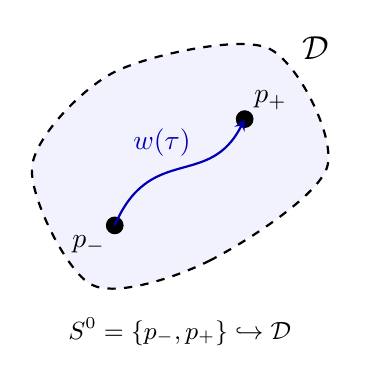
\begin{tikzpicture}[scale=1.5, >=stealth]
    % Draw region D
    \draw[thick, fill=blue!5, dashed] plot [smooth cycle] coordinates {(0,0) (1,0.2) (2,1) (1.5,2) (0.2,1.8) (-0.5,1)};
    \node at (1.9, 2.0) {\large $\mathcal{D}$};

    % Points p+ and p-
    \filldraw[black] (0.2, 0.5) circle (2pt) node[below left] {$p_-$};
    \filldraw[black] (1.3, 1.4) circle (2pt) node[above right] {$p_+$};

    % Path w
    \draw[thick, ->, blue!70!black] (0.2, 0.5) .. controls (0.5, 1.2) and (1.0, 0.8) .. (1.3, 1.4);
    \node[blue!70!black] at (0.6, 1.2) {$w(\tau)$};

    % Annotation
    \node[anchor=north] at (0.75, -0.2) {\small $S^0 = \{p_-, p_+\} \hookrightarrow \mathcal{D}$};
\end{tikzpicture}
\caption{\justifying \textbf{Topological embedding of the 0-sphere.}
The disconnected points $p_{\pm}$, representing the two internal energy kernels of the electron (kernel $A \equiv p_{-}$ and kernel $B \equiv p_{+}$), are embedded within an arcwise connected region $\mathcal{D}$. 
The region $\mathcal{D}$ is physically interpreted as a photon sphere: a three-dimensional confinement domain that supports internal radiative energy transport between the kernels. 
For illustrative clarity, $\mathcal{D}$ is depicted here as a two-dimensional planar region.
The continuous path $w(\tau)$ denotes a thermal geodesic along which thermal potential energy localized at kernel $A$ is converted into radiative energy, propagates through $\mathcal{D}$, and is absorbed at kernel $B$. 
This internal circulation induces a phase-dependent displacement of the internal energy center, whose motion follows a $\sin\theta$ dependence ($\theta=\omega t$), characteristic of simple harmonic motion.
The path $w(\tau)$ exists exclusively within the support provided by $\mathcal{D}$, reflecting the topological separation between discrete localization on $S^0$ and continuous transport in the embedding domain.
The explicit thermodynamic derivation of the $\sin\theta$-modulated internal motion from temperature-gradient-driven energy exchange is provided in Appendix~\ref{sec:internal_energy_dynamics}, in particular Section~\ref{subsec:sinusoidal_derivation}.}
\label{fig:embedding}


\end{figure}

It is important to emphasize that the embedding region $\mathcal{D}$ should be understood as a genuinely three-dimensional physical domain.
In the present work, $\mathcal{D}$ represents a photon sphere surrounding the electron, providing the spatial support for internal radiative energy transport.
The two-dimensional depiction in Fig.~\ref{fig:embedding} is adopted solely for topological clarity and visualization; no physical reduction of dimensionality is implied.
All topological statements made here—such as arcwise connectivity, existence of continuous paths, and deformation retraction in extreme limits—extend straightforwardly to the three-dimensional case.

The continuous transport within the embedding region $\mathcal{D}$ is not kinematically uniform.
As established in previous developments of the 0-Sphere model, the center-of-energy motion inside the photon sphere undergoes periodic acceleration and deceleration governed by a simple harmonic profile.
In particular, the effective energy flow along $w(\tau)$ follows a sinusoidal dependence on the internal phase parameter $\theta$, reflecting the internal redistribution of thermal potential energy between the two kernels.
The mathematical origin of this sinusoidal behavior is not postulated ad hoc but arises necessarily from the thermodynamic energy conservation and temperature-gradient structure of the dual-kernel system, as summarized in Appendix~\ref{sec:internal_energy_dynamics}.


% ========================================
% Section 4: Embedding into an Arcwise Connected Region
% ========================================
\section{Embedding into an Arcwise Connected Region}
\label{sec:embedding}

Within the physical interpretation of the 0-Sphere model, the points $p_{\pm}$ correspond to two internal energy kernels of the electron, denoted kernel $A$ and kernel $B$.
Thermal potential energy localized at a kernel represents rest mass energy in a fully phase-localized configuration.
Radiative transport between kernels occurs when thermal potential energy at kernel $A$ is converted into radiative energy, propagates along a thermal geodesic $w(\tau)$ within the photon sphere $\mathcal{D}$, and is subsequently absorbed at kernel $B$.
The kernels themselves remain fixed endpoints of the process; only energy propagates through $\mathcal{D}$.

Let $\mathcal{D} \subset \mathbb{R}^{n}$ be a compact, arcwise connected region \cite{Munkres2000} such that
\begin{equation}
i : S^{0} \hookrightarrow \mathcal{D}
\end{equation}
is an inclusion map. We refer to $\mathcal{D}$ as the admissible transport domain (photon sphere). By definition, for any two points $x,y \in \mathcal{D}$, there exists a continuous path
\begin{equation}
w : [0,1] \rightarrow \mathcal{D}, \qquad w(0)=x,\; w(1)=y .
\end{equation}
In particular, there exist paths in $\mathcal{D}$ connecting $p_{+}$ and $p_{-}$.

Crucially, these paths are elements of $\mathcal{D}$ and not of $S^{0}$.
The embedding region $\mathcal{D}$ therefore supplies the minimal geometrical structure required to support continuous transport, while preserving the discrete nature of the underlying localization (see Fig.~\ref{fig:embedding}).
In the physical interpretation, $\mathcal{D}$ represents a \textit{photon sphere}—a spatially confined region that contains both energy kernels and supports internal radiative circulation.

Physically, the continuous paths $w : [0,1] \rightarrow \mathcal{D}$ connecting kernel $A$ and kernel $B$ are not arbitrary curves but correspond to \textit{geodesics} determined by the principle of least action.
The radiative energy transport follows a refraction-like rule analogous to Snell's law in the internal phase space \cite{hanamura17765336}.
Along each infinitesimal segment $\delta s$ of the path within the photon sphere, the propagation angle varies continuously according to a differential form of Snell's law, reflecting local changes in the effective medium.
The kernels $A$ and $B$ remain fixed, while $v_A$ and $v_B$ denote the local propagation speeds of energy in the surrounding photon sphere adjacent to each kernel. The kernels themselves are fixed endpoints; the velocities refer to the local propagation of energy in the surrounding medium, not the motion of the kernels.

These infinitesimal variations accumulate smoothly, and applying the principle of least action over each $\delta s$ leads to a globally continuous geodesic connecting kernel $A$ and kernel $B$—the so-called ``thermal geodesic''~\cite{hanamura17765349}:
\begin{equation}
\frac{\sin \theta_A}{\sin \theta_B} = \frac{v_A}{v_B} \equiv n_{A \to B},
\end{equation}
where $\theta_A$ and $\theta_B$ denote the local propagation angles at the ends of each infinitesimal segment, and $v_A, v_B$ are the local propagation speeds within the photon sphere adjacent to the kernels.
The total path minimizes the integrated action
\begin{equation}
S = \int_{\text{kernel }A}^{\text{kernel }B} ds,
\end{equation}
subject to the fixed thermal energy boundary conditions at kernels $A$ and $B$.
This geodesic motion connects the quantum oscillations of the 0-Sphere model with the geometric principles underlying the present topological framework, ensuring that all energy circulates between the fixed kernels along admissible paths.


The characteristic spatial extent of $\mathcal{D}$ is on the order of the Compton wavelength, $\mathcal{O}(\lambda_C)$ where $\lambda_C = h/(mc)$, corresponding to the scale of radiation exchanged between kernel $A$ and kernel $B$ (see Appendix~\ref{sec:appendix_physical_scale} for numerical estimates).
No additional degrees of freedom are introduced on $S^{0}$ itself.

% ========================================
% Section 5: Topological Confinement of Thermal Potential Energy
% ========================================
\section{Topological Confinement of Thermal Potential Energy}
\label{sec:confinement}

Within this framework, thermal potential energy remains localized at the discrete kernels $p_{\pm}$ (Fig.~\ref{fig:embedding}), corresponding to rest mass energy $mc^2$ concentrated at kernel $A$ and kernel $B$.
Admissible transport between kernels is defined by continuous radiative paths supported in the photon sphere $\mathcal{D}$.
These paths are not arbitrary curves but geodesics satisfying the principle of least action \cite{hanamura17765336}, ensuring that radiative energy follows the physically realized trajectory that minimizes the action integral between the fixed kernel endpoints.
This radiative exchange follows Zitterbewegung oscillations derived from the Dirac equation, characterized by the internal phase evolution $\omega\tau$, where $\tau$ is the proper time.
Complete energy transfer from kernel $A$ to kernel $B$ requires the full radiation of rest mass energy initially localized at kernel $A$, with characteristic wavelength given by the Compton wavelength $\lambda_C = h/(mc)$.

Denoting the effective support of transport by $\mathrm{supp}(E)$, one has
\begin{equation}
\mathrm{supp}(E) \subset \mathcal{D}.
\end{equation}

\textbf{This inclusion expresses a purely geometrical constraint: all non-vanishing internal energy of the electron is confined to the photon-sphere domain $\mathcal{D}$.}
As a consequence, radiative energy circulates exclusively within $\mathcal{D}$ without dissipating into the external environment.
Continuous energy transport is therefore supported only inside $\mathcal{D}$, while the discrete energy kernels remain localized on $S^{0}$.

Since the inclusion map $i(S^{0})$ is disjoint from the complement $\mathbb{R}^{n}\setminus \mathcal{D}$, no continuous radiative path can extend beyond the boundary of $\mathcal{D}$.
The resulting confinement is thus topological rather than dynamical \cite{Geroch1970}: it does not rely on equations of motion, symmetry principles, or conserved currents, in contrast to standard treatments of energy localization \cite{Wald1984}.
Energy conservation consequently emerges as a geometric consequence of confinement, rather than as a dynamically imposed law.


\begin{figure}[t!]
\centering
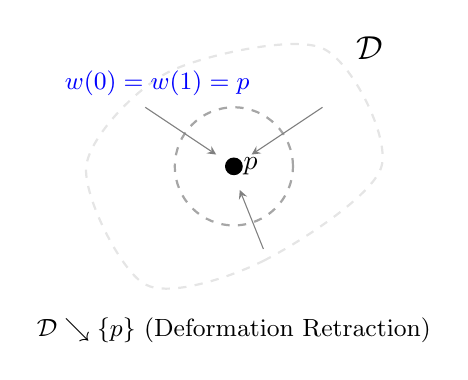
\begin{tikzpicture}[scale=1.5, >=stealth]
    % Contracting region D
    \draw[gray!20, thick, dashed] plot [smooth cycle] coordinates {(0,0) (1,0.2) (2,1) (1.5,2) (0.2,1.8) (-0.5,1)};
    \draw[gray!70, thick, dashed] (0.75, 1.0) circle (0.5);
    \node at (1.9, 2.0) {\large $\mathcal{D}$};
    
    % Center point p
    \filldraw[black] (0.75, 1.0) circle (2pt) node[right] {$p$};
    
    % Arrows indicating contraction
    \draw[->, gray] (1.5, 1.5) -- (0.9, 1.1);
    \draw[->, gray] (0.0, 1.5) -- (0.6, 1.1);
    \draw[->, gray] (1.0, 0.3) -- (0.8, 0.8);

    % Degenerate path
    \node[blue] at (0.1, 1.7) {\small $w(0)=w(1)=p$};

    % Annotation
    \node[anchor=north] at (0.75, -0.2) {\small $\mathcal{D} \searrow \{p\}$ (Deformation Retraction)};
\end{tikzpicture}
\caption{\justifying \textbf{Deformation retraction in the extreme limit.} As the embedding region $\mathcal{D}$ contracts to a single point $p$, all paths supported in $\mathcal{D}$ degenerate to constant maps, leading to the suppression of radiative transport.}
\label{fig:retraction}
\end{figure}


% ========================================
% Section 6: Extreme Limits and Degeneracy of Transport
% ========================================
\section{Extreme Limits and Degeneracy of Transport}
\label{sec:extreme}

In extreme regimes, such as formally infinite effective energy scales, the characteristic Compton wavelength associated with radiation tends toward zero.
In this limit, the physically relevant support of energy transport may shrink below any finite length scale.
The embedding region $\mathcal{D}$ can be understood as having a characteristic size comparable to the Compton wavelength, providing the geometric scale over which kernel-to-kernel circulation remains admissible.

Geometrically, this situation can be modeled by an effective collapse of the embedding region $\mathcal{D}$.
In particular, $\mathcal{D}$ may admit a deformation retraction (see Appendix~\ref{sec:appendix_deformation} for formal definition) \cite{Munkres2000} onto a single point $p$,
\begin{equation}
\mathcal{D} \;\searrow\; \{p\},
\end{equation}
rendering all continuous paths in $\mathcal{D}$ homotopically trivial (Fig.~\ref{fig:retraction}).
Consequently, any path $w$ supported in $\mathcal{D}$ degenerates to a constant map,
\begin{equation}
w(0)=w(1)=p .
\end{equation}

Within the 0-Sphere model, this degeneration corresponds to a suppression of radiative transport:
no nontrivial circulation between kernel $A$ and kernel $B$ can be supported once admissible paths collapse.
Importantly, this behavior does not signal a divergence of observable quantities.
Rather, it reflects a loss of admissible transport structures in the extreme limit.
This mechanism replaces dynamical blow-up with a loss of topological degrees of freedom, echoing modern geometric approaches to singularity resolution \cite{Penrose1965,Ashtekar2005}.


% ========================================
% Section 7: Discussion and Outlook
% ========================================
\section{Discussion and Outlook}
\label{sec:discussion}

By separating discrete localization from continuous transport, the present framework clarifies the internal logic of the 0-Sphere model.
Arcwise connectivity is attributed exclusively to the embedding region (the photon sphere $\mathcal{D}$), while the 0-sphere itself remains strictly disconnected.
This distinction prevents mathematical misinterpretation and provides a minimal geometrical basis for physically meaningful circulation between kernel $A$ and kernel $B$.
The term ``photon sphere'' is used here in a model-internal sense, distinct from its usage in classical general relativity.

Physically, the photon sphere $\mathcal{D}$ corresponds to a spatially confined region—on the order of the Compton wavelength—within which a single electron exists as a unified system.
The topological confinement condition $\mathrm{supp}(E) \subset \mathcal{D}$ ensures that thermal potential energy radiated from one kernel is completely absorbed by the other kernel without external dissipation.
This geometric constraint naturally preserves the energy conservation identity~\eqref{eq:energy_conservation}, demonstrating that conservation laws can emerge from topological structure rather than requiring dynamical imposition.
In this sense, the present framework may be viewed as an attempt to reinterpret quantum-mechanical descriptions not primarily in terms of static states, but in terms of admissible internal processes governed by geometric and topological constraints.
The resulting picture complements existing kinematic descriptions of internal oscillatory dynamics and phase accumulation by providing a coherent topological foundation for their physical realization.

It is also important to emphasize that the boundary $\partial \mathcal{D}$ in the present model should not be interpreted as a mere physical barrier.
Rather, it functions as a causal boundary in a geometric sense, delimiting the conditions under which continuous maps supporting admissible transport may exist.
The existence or absence of such admissible paths determines whether internal circulation is possible, independently of any local equations of motion.

From this perspective, divergences traditionally associated with singular limits need not be understood as the unbounded growth of physical quantities.
Instead, they may reflect a loss of available topological degrees of freedom, manifested here as the effective contractibility of the embedding region (Fig.~\ref{fig:retraction}).
Such behavior suggests that certain singular phenomena can be reinterpreted geometrically, as transitions in the space of admissible processes rather than as failures of dynamical laws.
This viewpoint offers a potential route by which singular behavior may be rendered non-divergent, without invoking additional dynamical mechanisms.

\clearpage

% ========================================
% Acknowledgments
% ========================================
\section*{Acknowledgments}
This work was conducted independently by the author. During preparation, large language models were used as a pedagogical and editorial aid, primarily to verify the standard presentation of well-established concepts in topology and differential geometry, and to improve the clarity and logical organization of the exposition. 
In particular, the models were consulted to cross-check the conventional definitions of topological structures such as discrete topology, arcwise connectivity, and deformation retraction, not to generate new physical content or interpretations. All physical assumptions, conceptual judgments, and the geometrical reinterpretation of energy confinement proposed here were formulated and assessed solely by the author.


% ========================================
% Bibliography
% ========================================
\begin{thebibliography}{9}

% ========================================
% Line Integral Trilogy
% ========================================

\bibitem{hanamura18067760}
S.~Hanamura, ``Geometric Structure of Spinorial Phase Accumulation along Thermal Geodesics,'' Zenodo (2025). \href{https://doi.org/10.5281/zenodo.18067760}{https://doi.org/10.5281/zenodo.18067760}
% Elucidates the geometric structure of spinorial phase accumulation via line integrals of the connection along thermal geodesics. Shows that a straight-line geodesic in real space internally accumulates a 2pi phase via the spinorial connection generated by Thomas precession, and establishes a correspondence with the Poincare upper half-plane.

\bibitem{hanamura18135855}
S.~Hanamura, ``From Curvature to Connection: Revisiting the Geometric Origin of Conservation Laws,'' Zenodo (2026). \href{https://doi.org/10.5281/zenodo.18135855}{https://doi.org/10.5281/zenodo.18135855}
% Reinterprets the Einstein field equations as a post-hoc consistency condition expressed via line integrals of the connection. Resolves the geometric derivation of conservation laws challenge shared by Weyl, Cartan, Palatini, and Ashtekar through the requirement of global consistency in phase accumulation along thermal geodesics.

\bibitem{hanamura18203433}
S.~Hanamura, ``Line Integrals as Fundamental Observables in Physics: A Unified Principle Behind the Aharonov--Bohm Effect, Berry Phase, and Wilson Loops,'' Zenodo (2026). \href{https://doi.org/10.5281/zenodo.18203433}{https://doi.org/10.5281/zenodo.18203433}
% Unifies observables in quantum, gauge, and gravitational theories as line integrals of the connection. Shows that the Aharonov-Bohm effect, Berry phase, and Wilson loops all rest on the same geometric principle (path-dependence, primacy of open paths), with a concrete realization via thermal gradients in the 0-Sphere dual-kernel system.

% ========================================

\bibitem{hanamura17765336}
S.~Hanamura,
``From Zero-Sphere to Emergent Spacetime: A Minimalist Background-Independent Framework for Temporal and Spatial Genesis,''
Zenodo (2025).
\href{https://doi.org/10.5281/zenodo.17765336}{DOI: 10.5281/zenodo.17765336}

\bibitem{hanamura17765136}
S.~Hanamura,
``From Clock Synchronization to Electromagnetism: A Realist Construction of U(1) Gauge Theory,''
Zenodo (2025).
\href{https://doi.org/10.5281/zenodo.17765136}{DOI: 10.5281/zenodo.17765136}

\bibitem{hanamura17764997}
S.~Hanamura,
``Redefining Electron Spin and Anomalous Magnetic Moment Through Harmonic Oscillation and Lorentz Contraction,''
Zenodo (2024).
\href{https://doi.org/10.5281/zenodo.17764997}{DOI: 10.5281/zenodo.17764997}

\bibitem{Schrodinger1930}
E.~Schrödinger,
``Über die kräftefreie Bewegung in der relativistischen Quantenmechanik,''
Sitzungsber. Preuss. Akad. Wiss. Phys. Math. Kl. \textbf{24}, 418 (1930).

\bibitem{Thaller1992}
B.~Thaller,
\textit{The Dirac Equation}
(Springer-Verlag, Berlin, 1992).
\href{https://doi.org/10.1007/978-3-662-02753-9}{DOI: 10.1007/978-3-662-02753-9}

\bibitem{Frankel2011}
T.~Frankel,
\textit{The Geometry of Physics},
3rd ed. (Cambridge University Press, 2011).  
DOI: 10.1017/CBO9781139061377

\bibitem{Geroch1970}
R.~Geroch,
``Topology in General Relativity,''
J. Math. Phys. \textbf{11}, 437 (1970).  
DOI: 10.1063/1.1665157

\bibitem{hanamura18275142}
S.~Hanamura, ``Dissolution of the Vacuum Energy Problem in an Integral-Based Ontology: the 0-Sphere Model Perspective,'' Zenodo (2026). \href{https://doi.org/10.5281/zenodo.18275142}{https://doi.org/10.5281/zenodo.18275142}

\bibitem{Munkres2000}
J.~R.~Munkres,
\textit{Topology},
2nd ed. (Prentice Hall, 2000).  
\href{https://www.pearson.com/en-us/subject-catalog/p/topology/P200000003295}{Publisher link}

\bibitem{hanamura17765349}
S.~Hanamura, ``Thermal Geodesics in the 0-Sphere Model: Extending General Relativity Through Internal Thermodynamic Structure,'' Zenodo (2025). \href{https://doi.org/10.5281/zenodo.17765349}{https://doi.org/10.5281/zenodo.17765349}

\bibitem{Wald1984}
R.~M.~Wald,
\textit{General Relativity}
(University of Chicago Press, 1984).  
\href{https://press.uchicago.edu/ucp/books/book/chicago/G/bo3684313.html}{Publisher link}

\bibitem{Penrose1965}
R.~Penrose,
``Gravitational Collapse and Space-Time Singularities,''
Phys. Rev. Lett. \textbf{14}, 57 (1965).  
DOI: 10.1103/PhysRevLett.14.57

\bibitem{Ashtekar2005}
A.~Ashtekar and M.~Bojowald,
``Quantum Geometry and the Schwarzschild Singularity,''
Class. Quantum Grav. \textbf{23}, 391 (2006).  
DOI: 10.1088/0264-9381/23/2/008

\bibitem{hanamura17765409}
S.~Hanamura, ``Spin from Geometry: Emergence of Spin via Internal Berry Phase in the 0-Sphere Electron Model,'' Zenodo (2025). \href{https://doi.org/10.5281/zenodo.17765409}{https://doi.org/10.5281/zenodo.17765409}

\bibitem{hanamura16759284} 
S. Hanamura, A Model of an Electron Including Two Perfect Black Bodies, Zenodo (2018), \href{https://doi.org/10.5281/zenodo.16759284}{doi:10.5281/zenodo.16759284}. [Originally: \href{https://vixra.org/abs/1811.0312}{viXra:1811.0312}]

\bibitem{hanamura17765097}
S.~Hanamura, ``Bridging Quantum Mechanics and General Relativity: A First-Principles Approach to Anomalous Magnetic Moments and Geodetic Precession,'' Zenodo (2025). \href{https://doi.org/10.5281/zenodo.17765097}{https://doi.org/10.5281/zenodo.17765097}

\bibitem{hanamura17760132}
S.~Hanamura, ``Coexistence Positive and Negative-Energy States in the Dirac Equation with One Electron,'' Zenodo (2020). \href{https://doi.org/10.5281/zenodo.17760132}{https://doi.org/10.5281/zenodo.17760132}

\end{thebibliography}

\clearpage


\appendix


% ========================================
% Appendix A: What is the 0-sphere
% ========================================
\section{What is the 0-sphere}
\label{sec:what_is_the_0_sphere}

A 0-sphere ($S^0$) is the simplest object in the hierarchy of $n$-spheres.
Topologically, it consists of exactly two disconnected points and carries no notion of length, area, or volume.
In contrast to higher-dimensional spheres, $S^0$ possesses no internal continuity; its defining feature is discreteness.

To build geometric intuition, it is useful to compare the 0-sphere with the 1-sphere ($S^1$), as illustrated in Fig.~\ref{fig:s0_s1_comparison}.
Panel~(a) depicts a 0-sphere as a pair of points located at $x=\pm a$ on a one-dimensional line.
These points can be interpreted as the intersection of a straight line with a circle (or, equivalently, a hollow sphere embedded in higher dimensions).
From this perspective, the 0-sphere emerges not as an extended object, but as a set of isolated boundary points defined by a global geometric constraint.

Panel~(b) shows a 1-sphere, which is a continuous closed curve.
Unlike $S^0$, the 1-sphere admits continuous paths along its circumference, allowing intrinsic notions of distance and angular displacement.
This contrast highlights a fundamental distinction: while $S^1$ supports continuous motion within itself, $S^0$ does not.
Any notion of transport or interaction between the two points of a 0-sphere must therefore be mediated by an external embedding space.

This distinction is central to the 0-Sphere electron model.
The two points of $S^0$ are interpreted as discrete internal energy kernels, while all continuous processes—such as radiative transport, thermal gradients, and virtual photon propagation—occur in an embedding domain that surrounds and supports the 0-sphere.
In the main text, this embedding domain is identified with the photon sphere $\mathcal{D}$, within which continuous thermal geodesics exist.
The separation between discrete localization on $S^0$ and continuous dynamics in $\mathcal{D}$ underlies the topological origin of internal oscillatory motion discussed throughout this paper.

\begin{figure}[t!]
    \centering
    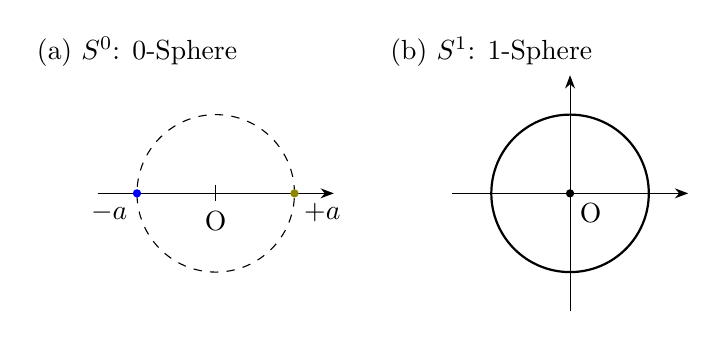
\begin{tikzpicture}[>=Stealth, scale=1.0]

        % --- (a) S^0: 0-Sphere ---
        \begin{scope}[shift={(0,0)}]
            \node at (-1, 1.8) {\normalsize (a) $S^0$: 0-Sphere};
            
            % Axis
            \draw[->] (-1.5,0) -- (1.5,0);
            
            % Dashed circle
            \draw[dashed] (0,0) circle (1);
            
            % Center O
            \draw (0,-0.1) -- (0,0.1) node[below=6pt] {O};
            
            % Points -a and +a
            \fill[blue] (-1,0) circle (1.5pt) node[below left, black] {$-a$};
            \fill[olive] (1,0) circle (1.5pt) node[below right, black] {$+a$};
        \end{scope}

        % --- (b) S^1: 1-Sphere ---
        \begin{scope}[shift={(4.5,0)}]
            \node at (-1, 1.8) {\normalsize (b) $S^1$: 1-Sphere};
            
            % Coordinate axes
            \draw[->] (-1.5,0) -- (1.5,0);
            \draw[->] (0,-1.5) -- (0,1.5);
            
            % Solid circle
            \draw[thick] (0,0) circle (1);
            
            % Center O
            \fill (0,0) circle (1.5pt) node[below right] {O};
        \end{scope}

    \end{tikzpicture}
    \caption{\justifying \textbf{Geometric comparison of the 0-sphere and 1-sphere.}
    (a) The 0-sphere $S^0$ consists of two disconnected points located at $x=\pm a$, which may be viewed as the intersection of a line with a circle.
    Despite the presence of a surrounding geometric constraint (dashed circle), $S^0$ itself contains no continuous paths.
    (b) The 1-sphere $S^1$ is a continuous closed curve admitting intrinsic angular motion.
    This contrast emphasizes that any continuous transport between the two points of $S^0$ must occur in an external embedding domain rather than on the sphere itself.}
    \label{fig:s0_s1_comparison}
\end{figure}

\begin{figure}[t!]
    \centering
    \resizebox{0.95\columnwidth}{!}{%
        % fig_thermal.tex
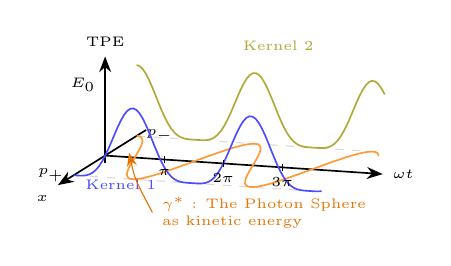
\begin{tikzpicture}[
    % Unit length for coordinate axes
    x={(0.75cm,-0.05cm)},   % wt axis
    y={(0cm,0.9cm)},        % TPE axis
    z={(-0.4cm,-0.25cm)},   % x axis
    >=Stealth
]
    % --- Guide lines ---
    \draw[gray!30, dashed, thin] (0,0,1) -- (4.2,0,1);  % +a
    \draw[gray!30, dashed, thin] (0,0,-1) -- (4.2,0,-1); % -a

    % Font sizes in decreasing order: \small, \footnotesize, \scriptsize, \tiny
    % --- Coordinate axes ---
    \draw[semithick, ->] (0,-0.1,0) -- (0,1.4,0) node[above, font=\tiny] {TPE};
    \node[left, font=\tiny] at (0,1,0) {$E_0$};
    
    \draw[semithick, ->] (0,0,0) -- (4.7,0,0) node[right, font=\tiny] {$\omega t$};
    
    \draw[semithick, ->] (0,0,-1.3) -- (0,0,1.5) node[below left, font=\tiny] {$x$};
    \node[left, font=\tiny] at (0,0,1) {$p_{+}$};
    \node[right, font=\tiny] at (0,0,-1) {$p_{-}$};
    
    % --- Function plots ---
    % 1. Orange (Photon Sphere): oscillates between p_{-} and p_{+}
    \draw[orange!80, semithick, domain=0:4.2, samples=80] 
        plot (\x, 0, {-1 * cos(\x * 180)});
    
    % 2. Blue (Kernel 1): on the x = +a plane
    \draw[blue!70, semithick, domain=0:4.2, samples=80] 
        plot (\x, {sin(\x * 90)^4}, 1);
    % Label placed at position (wt=0.8, TPE=-0.3, x=+a)
    \node[blue!70, font=\tiny, anchor=south] at (0.8, -0.3, 1) {Kernel 1};
    
    % 3. Olive (Kernel 2): on the x = -a plane
    \draw[olive!70, semithick, domain=0:4.2, samples=80] 
        plot (\x, {cos(\x * 90)^4}, -1);
    \node[olive!70, font=\tiny, anchor=south] at (2.4, 1.2, -1) {Kernel 2};
    
    % --- Tick labels ---
    \foreach \x/\label in {1/\pi, 2/2\pi, 3/3\pi} {
        \draw (\x, 0.05, 0) -- (\x, -0.05, 0);
        \node[below, font=\tiny] at (\x, 0, 0) {$\label$};
    }
    
    % --- Sphere at origin (commented out) ---
    %\fill[yellow!40, opacity=0.5] (0,0,0) circle (0.15);
    %\shade[ball color=yellow!40, opacity=0.4] (0,0,0) circle (0.15);
    
    % --- Text annotation ---
    \node[orange!90!black, anchor=north west, align=left, font=\tiny] (text) at (0.8, -0.4, 0) {
        $\gamma^*$ : The Photon Sphere \\
        as kinetic energy
    };
    \draw[->, orange!90!black, thin] (text.west) .. controls (0.5,-0.3, 0) .. (0.3, 0, -0.2);
\end{tikzpicture}%
    }
    \caption{\justifying patiotemporal energy distribution within a single electron. The blue line (Kernel 1) and olive line (Kernel 2) show the alternating energy exchange between the two kernels positioned at $x = \pm a$. The orange curve ($\gamma^*$) represents the virtual photon oscillating spatially between these kernels. The conservation law $T_{\mathrm{e1}} + T_{\mathrm{e2}} + \gamma^*_{\mathrm{kinetic}} = E_0$ is maintained as the thermal energy gradient drives the internal dynamics.
    }
    \label{fig:appendix_virtual_photon}
\end{figure}


% ========================================
% Appendix B: Thermal energy gradient caused by two kernels
% ========================================
\section{Thermal energy gradient caused by two kernels}
\label{sec:thermal_energy_gradient}

In the 0-Sphere electron model, the internal dynamics are governed by energy exchange between two discrete kernels associated with the 0-sphere.
Each kernel alternates between the roles of emitter and absorber, ensuring strict conservation of total internal energy.
This subsection provides a physical explanation of how a time-dependent thermal energy gradient naturally arises between the two kernels and why it leads to sinusoidal internal motion.

Let the two kernels be characterized by thermal potential energies $T_{\mathrm{e1}}$ and $T_{\mathrm{e2}}$, respectively.
To satisfy energy conservation while allowing continuous energy circulation, the thermal energies are assigned complementary time dependences of the form
\begin{equation}
\begin{split}
T_{\mathrm{e1}} &= E_0 \cos^4\!\left(\frac{\theta}{2}\right), \\
T_{\mathrm{e2}} &= E_0 \sin^4\!\left(\frac{\theta}{2}\right),
\end{split}
\label{eq:kernel_temperatures}
\end{equation}
where $E_0$ denotes the ground-state internal energy and $\theta=\omega t$ is the phase of the internal cycle.
The quartic dependence reflects the black-body nature of thermal radiation emitted and absorbed by the kernels.

Because the kernels are spatially fixed points of the 0-sphere, spatial derivatives vanish identically.
The relevant gradient driving internal motion is therefore temporal in origin and is defined by the difference
\begin{equation}
\mathrm{grad}\,T_{\mathrm{e}} \equiv \frac{d}{d\theta}\left(T_{\mathrm{e2}} - T_{\mathrm{e1}}\right).
\end{equation}
Evaluating this expression yields the remarkably simple result
\begin{equation}
\mathrm{grad}\,T_{\mathrm{e}} = E_0 \sin\theta .
\label{eq:thermal_gradient_sine}
\end{equation}

Equation~\eqref{eq:thermal_gradient_sine} demonstrates that the thermal energy gradient between the two kernels varies sinusoidally in time.
This gradient acts as the driving source for internal radiative transport within the embedding domain, accelerating and decelerating the circulating radiative energy in a manner identical to that of a simple harmonic oscillator.
Importantly, the $\sin\theta$ dependence is not imposed as an assumption but emerges uniquely from the complementary thermal evolution of the two kernels.

The physical picture corresponding to this process is illustrated in Fig.~\ref{fig:appendix_virtual_photon}.
As shown there, the two kernels remain fixed while the virtual photon (radiative energy carrier) oscillates spatially between them under the action of the thermal energy gradient.
During this motion, the sum of the thermal potential energies of the kernels and the kinetic energy of the virtual photon remains constant, preserving the internal energy conservation law.
The sinusoidal displacement of the virtual photon directly reflects the $\sin\theta$ dependence of the driving thermal gradient.

Physically, thermal potential energy localized at one kernel is converted into radiative energy, propagates through the photon sphere embedding domain, and is subsequently absorbed by the opposite kernel.
The alternating dominance of $T_{\mathrm{e1}}$ and $T_{\mathrm{e2}}$ produces a periodic displacement of the internal energy center, giving rise to the sinusoidal internal motion employed throughout the main text.

It is important to emphasize that the discrete kernels themselves are not persistent spatial entities.
For a bound electron, the internal oscillation may appear as a simple harmonic motion about a fixed location.
However, for a free electron undergoing translational motion, a kernel localized at a given position does not reappear at the same spatial point after one oscillation cycle.
Instead, the sequence of localization follows $A \rightarrow B \rightarrow A'$, where $A' \neq A$, tracing the electron worldline through spacetime.
In this sense, individual kernel localizations vanish and re-emerge, while the history of internal energy transport is preserved as a line integral along the admissible radiative paths.


The detailed thermodynamic and mathematical derivation of the $\sin\theta$-modulated motion, including its relation to energy conservation and internal kinetic energy, is presented in Appendix~\ref{sec:internal_energy_dynamics}.
Here, the emphasis is on the physical origin of the driving gradient and its direct connection to the discrete two-kernel structure of the 0-sphere.


% ----------------------------------------
% Table 1: Hierarchy of Compton Wavelength Scales
% ----------------------------------------
\begin{table*}[t!]
\centering
\caption{Hierarchy of Compton wavelength scales and their physical roles.}
\label{tab:compton_wavelength_hierarchy}
\renewcommand{\arraystretch}{1.4}
\begin{tabular}{p{6.0cm}p{6.0cm}p{5.0cm}}
\toprule
\textbf{Quantity} & \textbf{Expression} & \textbf{Value (m)} \\
\midrule
Standard Compton wavelength
& $\lambda_C = \dfrac{h}{mc}$
& $2.426 \times 10^{-12}$ \\
\addlinespace[0.25cm]

Reduced Compton wavelength
& $\bar{\lambda}_C = \dfrac{\hbar}{mc} = \dfrac{\lambda_C}{2\pi}$
& $3.86 \times 10^{-13}$ \\
\addlinespace[0.25cm]

Zitterbewegung amplitude
& $\lambda_{ZB} = \dfrac{\hbar}{2mc} = \dfrac{\lambda_C}{4\pi}$
& $1.93 \times 10^{-13}$ \\
\addlinespace[0.20cm]
\bottomrule
\end{tabular}

\vspace{0.4em}
\begin{minipage}{0.95\textwidth}
\justifying\small
The conversion relations $\bar{\lambda}_C = \lambda_C/(2\pi)$ and
$\lambda_{ZB} = \lambda_C/(4\pi)$ follow directly from the definitions.
Here, $\lambda_{ZB}$ reflects the amplitude of the oscillatory term in the Dirac position operator,
whereas $\lambda_C$ serves as the global length scale defining the photon sphere $\mathcal{D}$
and the characteristic distance for inter-kernel energy transport.
\end{minipage}
\end{table*}


% ========================================
% Appendix C: On Continuous Maps from Connected Domains to the 0-Sphere
% ========================================
\section{On Continuous Maps from Connected Domains to the 0-Sphere}
\label{sec:appendix_continuous}

For completeness, we briefly recall a standard topological result underlying the discussion in Sec.~\ref{sec:zerosphere}.
Let $S^{0}=\{p_{+},p_{-}\}$ be equipped with the discrete topology, and let $[0,1]$ carry the standard topology.

\medskip
\noindent\textbf{Claim.}
Any continuous map $f:[0,1]\to S^{0}$ is necessarily constant.

\medskip
\noindent\textit{Explanation.}
Since $S^{0}$ is endowed with the discrete topology, the singleton sets $\{p_{+}\}$ and $\{p_{-}\}$ are open.
If $f$ were not constant, there would exist $t_{1},t_{2}\in[0,1]$ such that
$f(t_{1})=p_{+}$ and $f(t_{2})=p_{-}$.
By continuity, the inverse images $f^{-1}(\{p_{+}\})$ and $f^{-1}(\{p_{-}\})$ are open, nonempty, disjoint subsets of $[0,1]$ whose union is the entire interval.
This would imply that $[0,1]$ is disconnected, contradicting its well-known connectedness.
Hence $f$ must be constant.

\medskip
This result expresses the fact that the 0-sphere itself cannot support nontrivial continuous paths.
In the present model, this observation motivates the introduction of an embedding region that provides the minimal geometric structure required for admissible transport.

% ========================================
% Appendix D: Deformation Retraction: Formal Definition
% ========================================
\section{Deformation Retraction: Formal Definition}
\label{sec:appendix_deformation}

For the discussion in Sec.~\ref{sec:extreme}, we recall the notion of deformation retraction.

\medskip
\noindent\textbf{Definition.}
Let $\mathcal{D}$ be a topological space and $\{p\} \subset \mathcal{D}$ a subspace consisting of a single point. A \textit{deformation retraction} of $\mathcal{D}$ onto $\{p\}$ is a continuous map
\begin{equation}
H : \mathcal{D} \times [0,1] \to \mathcal{D}
\end{equation}
satisfying:
\begin{enumerate}
\item $H(x,0) = x$ for all $x \in \mathcal{D}$ (identity at $t=0$),
\item $H(x,1) = p$ for all $x \in \mathcal{D}$ (collapse at $t=1$),
\item $H(p,t) = p$ for all $t \in [0,1]$ (fixed point throughout).
\end{enumerate}

% The condition H(x,1) = p is the defining clause of deformation retraction: every point x in D is mapped to the single point p at parameter t=1. This states only the topological fact that the entire space D is continuously contracted to the single point p.


\medskip
\noindent\textit{Geometric interpretation.}
The map $H$ provides a continuous one-parameter family of maps $h_t(x) = H(x,t)$ that continuously deforms $\mathcal{D}$ into the single point $p$ while keeping $p$ itself fixed. As $t$ progresses from $0$ to $1$, the entire space $\mathcal{D}$ contracts to $p$.

The deformation retraction discussed here represents an exceptional limiting case in which the embedding domain loses its capacity to support transport, and should not be interpreted as describing generic internal motion of a free electron.


\medskip
\noindent\textbf{Physical significance in the 0-Sphere model.}
In the extreme limit discussed in Sec.~\ref{sec:extreme}, the embedding region $\mathcal{D}$ (photon sphere) undergoes such a deformation retraction as the effective energy scale increases and the Compton wavelength $\lambda_C \to 0$. During this process, all continuous paths $w : [0,1] \to \mathcal{D}$ connecting the kernels degenerate to constant maps, suppressing radiative transport without causing divergences in observable quantities.

% ========================================
% Appendix E: Physical Scale of the Photon Sphere
% ========================================
\section{Physical Scale of the Photon Sphere}
\label{sec:appendix_physical_scale}

The characteristic spatial extent of the photon sphere $\mathcal{D}$ is on the order of the Compton wavelength, $\mathcal{O}(\lambda_C)$, where $\lambda_C = h/(mc)$ is associated with the electron.

\medskip
\noindent\textbf{Numerical estimate.}
For the electron with mass $m_e = 9.109 \times 10^{-31}$ kg, the Compton wavelength is
\begin{equation}
\lambda_C = \frac{h}{m_e c} \approx 2.426 \times 10^{-12} \text{ m} = 2.426 \text{ pm}.
\end{equation}
This sets the spatial scale over which kernel-to-kernel energy transport occurs.

\medskip
\noindent\textbf{Zitterbewegung frequency.}
Recent analysis of the anomalous magnetic moment through Lorentz contraction of rotational motion predicts that the actual velocity of internal oscillation is not the speed of light but approximately $\beta = v/c \approx 0.04047$ \cite{hanamura17764997}.
The internal oscillation frequency $\nu$ appearing in the energy conservation identity \eqref{eq:energy_conservation} is therefore
\begin{equation}
\begin{split}
\nu &= \frac{\beta c}{\lambda_C} \\
    &= \frac{0.04047 \times 299792458 \text{ m/s}}{2.42631 \times 10^{-12} \text{ m}} \\
    &\approx 5.007 \times 10^{18} \text{ Hz},
\end{split}
\end{equation}
corresponding to an angular frequency $\omega = 2\pi\nu \approx 3.146 \times 10^{19}$ rad/s.
This corresponds to a characteristic time scale $\tau_C = 2\pi/\omega \approx 2.00 \times 10^{-19}$ s, which is the proper time for one complete oscillation cycle between kernel $A$ and kernel $B$.
This prediction differs significantly from the traditional Zitterbewegung frequency based on $v = c$, and reflects the physical constraint that the average velocity of energy circulation within the photon sphere is substantially less than the speed of light.

\medskip
\noindent\textbf{Geometric confinement domain.}
The photon sphere $\mathcal{D}$ can be understood as a region of diameter $\mathcal{O}(\lambda_C)$ centered on the electron's center of mass. The topological constraint $\mathrm{supp}(E) \subset \mathcal{D}$ ensures that radiative energy exchange between the kernels remains confined to this Compton-scale region, preventing external dissipation and preserving the energy conservation identity.


% ========================================
% Appendix F: Compton Wavelength Scales in Zitterbewegung
% ========================================
\section{Compton Wavelength Scales in Zitterbewegung}
\label{sec:appendix_zb_scales}

The characteristic length scales associated with Zitterbewegung (trembling motion) require careful distinction between several related quantities. This appendix clarifies the hierarchy of Compton wavelength scales and their physical origins.

% ----------------------------------------
% Subsection F.1: Three Compton Wavelength Definitions
% ----------------------------------------
\subsection{Three Compton Wavelength Definitions}

\noindent\textbf{Standard Compton wavelength:}
\begin{equation}
\lambda_C = \frac{h}{mc} \approx 2.426 \times 10^{-12} \text{ m}
\end{equation}

\noindent\textbf{Reduced Compton wavelength:}
\begin{equation}
\bar{\lambda}_C = \frac{\hbar}{mc} = \frac{\lambda_C}{2\pi} \approx 3.86 \times 10^{-13} \text{ m}
\end{equation}

\noindent\textbf{Zitterbewegung amplitude:}
\begin{equation}
\lambda_{ZB} = \frac{\hbar}{2mc} = \frac{\bar{\lambda}_C}{2} = \frac{\lambda_C}{4\pi} \approx 1.93 \times 10^{-13} \text{ m}
\end{equation}



% ----------------------------------------
% Subsection F.2: Physical Origin of the Factor 1/2
% ----------------------------------------
\subsection{Physical Origin of the Factor 1/2}

The Zitterbewegung amplitude $\lambda_{ZB}$ is smaller than the reduced Compton wavelength $\bar{\lambda}_C$ by a factor of 2. This factor has three complementary physical interpretations:

\medskip
\noindent\textbf{1. Energy gap and angular frequency.}

Zitterbewegung arises from interference between positive-energy ($E > 0$) and negative-energy ($E < 0$) states in the Dirac equation. The energy gap between these states is
\begin{equation}
\Delta E = 2mc^2,
\end{equation}
leading to an angular frequency
\begin{equation}
\omega_{zb} = \frac{\Delta E}{\hbar} = \frac{2mc^2}{\hbar}.
\end{equation}

For oscillatory motion with velocity $v \approx c$ and angular frequency $\omega_{zb}$, the amplitude is
\begin{equation}
A_{zb} \approx \frac{c}{\omega_{zb}} = \frac{c}{2mc^2/\hbar} = \frac{\hbar}{2mc} = \lambda_{ZB}.
\end{equation}

The factor of 2 in the denominator originates directly from the energy gap $2mc^2$ between positive and negative energy states.

\medskip
\noindent\textbf{2. Position operator expectation value.}

In the Dirac theory, the time evolution of the position operator contains a rapidly oscillating term:
\begin{equation}
x(t) = x_{\text{classical}}(t) + \frac{i\hbar c}{2} \left(\alpha(0) - cp H^{-1}\right) e^{-2iHt/\hbar} H^{-1},
\end{equation}
where $\alpha$ are the Dirac matrices and $H$ is the Hamiltonian. The coefficient $1/2$ appears explicitly in the oscillatory term, determining the amplitude of the high-frequency fluctuation.

\medskip
\noindent\textbf{3. Spin angular momentum correspondence.}

In semiclassical models of Zitterbewegung as circular motion at speed $c$ with radius $R$, the angular momentum is
\begin{equation}
L = mRc.
\end{equation}

Equating this to the electron spin $S = \hbar/2$ gives
\begin{equation}
\frac{\hbar}{2} = mRc \quad \Rightarrow \quad R = \frac{\hbar}{2mc} = \lambda_{ZB}.
\end{equation}

The spin magnitude $\hbar/2$ (not $\hbar$) directly determines the factor of 2 in the Zitterbewegung amplitude. This correspondence should be understood as a semiclassical consistency argument rather than a derivation within the Dirac theory itself. The hierarchy of these length scales, their numerical values, and physical roles are summarized in Table~\ref{tab:compton_wavelength_hierarchy}.


% ----------------------------------------
% Subsection F.3: Application to the 0-Sphere Model
% ----------------------------------------
\subsection{Application to the 0-Sphere Model}

In the present topological framework, the following usage hierarchy applies:

\begin{enumerate}
\item \textbf{General discussions:} Use the order-of-magnitude expression $\mathcal{O}(\lambda_C)$ when describing the spatial extent of the photon sphere or characteristic transport distances, where factors of $2\pi$ are immaterial at the level of geometric order-of-magnitude estimates.

\item \textbf{Detailed Zitterbewegung calculations:} Use the specific amplitude $\lambda_{ZB} = \lambda_C/(4\pi)$ when precise analysis of internal oscillation requires explicit length scales.

\item \textbf{Velocity and frequency predictions:} Use the 0-Sphere model predictions $\beta = 0.04047$ and $\nu \approx 5.007 \times 10^{18}$ Hz, derived from the anomalous magnetic moment through Lorentz contraction of rotational motion \cite{hanamura17764997}. These frequencies are distinct from the Dirac Zitterbewegung frequency $\omega_{zb}/(2\pi) = mc^2/(\pi\hbar)$ and arise from a different, model-specific dynamical mechanism.
\end{enumerate}

The distinction between $\mathcal{O}(\lambda_C)$ (general scale), $\lambda_{ZB}$ (specific Dirac amplitude), and the velocity prediction $\beta = 0.04047$ (derived from experiment) maintains clarity between geometric approximations and quantitative physical predictions.

% ========================================
% Appendix G: Length Scale Selection in Frequency Predictions
% ========================================
\section{Length Scale Selection in Frequency Predictions}
\label{sec:appendix_scale_selection}

This appendix provides a reference calculation using the Zitterbewegung amplitude $\lambda_{ZB}$, solely for comparison with the Compton-scale estimate employed in the main text. It does not represent the physical scale adopted in the 0-Sphere model.

The choice of length scale in oscillation frequency calculations has significant physical implications. This appendix clarifies why $\lambda_C$ (standard Compton wavelength) is used in the 0-Sphere model predictions rather than $\lambda_{ZB}$ (Zitterbewegung amplitude).


% ----------------------------------------
% Table 2: Frequency Predictions Using Different Length Scales
% ----------------------------------------
\begin{table}[t!]
\caption{Frequency predictions using different length scales}
\label{tab:frequency_scale_comparison}
\centering
\begin{tabular}{lccc}
\toprule
\textbf{Length scale} & \textbf{Value (m)} & \textbf{Frequency (Hz)} & \textbf{Regime} \\
\midrule
\addlinespace[0.25cm]
$\lambda_C$ & $2.426 \times 10^{-12}$ & $5.007 \times 10^{18}$ & X-ray \\
\addlinespace[0.25cm]
$\lambda_{ZB}$ & $1.93 \times 10^{-13}$ & $6.29 \times 10^{19}$ & Gamma-ray \\
\addlinespace[0.25cm]
\midrule
\multicolumn{4}{l}{Ratio: $\nu_{ZB}/\nu_C = 4\pi \approx 12.57$} \\
\bottomrule
\end{tabular}
\par\vspace{0.3em}
\begin{minipage}{\columnwidth}
\justifying\small
The choice of length scale changes the predicted frequency by a factor of $4\pi$, shifting the electromagnetic regime from X-ray to gamma-ray.
\end{minipage}
\end{table}

% ----------------------------------------
% Subsection G.1: Comparison of Frequency Predictions
% ----------------------------------------
\subsection{Comparison of Frequency Predictions}

\noindent\textbf{Using standard Compton wavelength $\lambda_C$:}
\begin{equation}
\begin{split}
\nu_C &= \frac{\beta c}{\lambda_C} \\
      &= \frac{0.04047 \times 299792458 \text{ m/s}}{2.42631 \times 10^{-12} \text{ m}} \\
      &\approx 5.007 \times 10^{18} \text{ Hz}
\end{split}
\end{equation}

\noindent\textbf{Using Zitterbewegung amplitude $\lambda_{ZB}$:}
\begin{equation}
\begin{split}
\nu_{ZB} &= \frac{\beta c}{\lambda_{ZB}} = \frac{\beta c}{\lambda_C/(4\pi)} = 4\pi \cdot \frac{\beta c}{\lambda_C} \\
         &= \frac{0.04047 \times 299792458 \text{ m/s}}{1.93 \times 10^{-13} \text{ m}} \\
         &\approx 6.29 \times 10^{19} \text{ Hz}
\end{split}
\end{equation}

The numerical consequences of this scale choice are summarized in Table~\ref{tab:frequency_scale_comparison}.
The table makes explicit how the selection of the characteristic length scale directly shifts the predicted oscillation frequency by a factor of $4\pi$, thereby moving the relevant electromagnetic regime from X-ray to gamma-ray energies.
This comparison is provided to clarify the physical meaning of the scale selection adopted in the main text, rather than to suggest an alternative operating regime for the 0-Sphere model.


% ----------------------------------------
% Subsection G.2: Physical Interpretation and Scale Selection
% ----------------------------------------
\subsection{Physical Interpretation and Scale Selection}

The factor of $4\pi$ difference arises from the distinct physical roles of these length scales:

\medskip
\noindent\textbf{$\lambda_C$ (Standard Compton wavelength):}
\begin{itemize}
\item Represents the global scale of the photon sphere $\mathcal{D}$
\item Characterizes the overall kernel-to-kernel transport distance
\item Relevant for energy conservation identity \eqref{eq:energy_conservation} involving total energy circulation between kernels A and B
\item Describes the macroscopic confinement region
\end{itemize}

\medskip
\noindent\textbf{$\lambda_{ZB}$ (Zitterbewegung amplitude):}
\begin{itemize}
\item Represents the amplitude of the oscillatory term in the Dirac position operator
\item Describes the local high-frequency fluctuation around each kernel
\item Relevant for internal microstructure within each localized energy state
\item Not the characteristic scale for inter-kernel energy transport
\end{itemize}

% ----------------------------------------
% Subsection G.3: Justification for Using lambda_C
% ----------------------------------------
\subsection{Justification for Using $\lambda_C$}

In the present topological framework, $\lambda_C$ is the appropriate choice because:

\begin{enumerate}
\item \textbf{Energy transport scale:} the 0-Sphere model describes average energy circulation between discrete kernels separated by distances $\mathcal{O}(\lambda_C)$, not high-frequency position fluctuations within a single kernel.

\item \textbf{Photon sphere geometry:} The topological constraint $\mathrm{supp}(E) \subset \mathcal{D}$ operates at the scale of the entire confinement region, with diameter $\mathcal{O}(\lambda_C)$.

\item \textbf{Physical regime consistency:} The predicted frequency $\nu \approx 5.007 \times 10^{18}$ Hz (X-ray regime) is consistent with Compton-scale physics. Using $\lambda_{ZB}$ would yield $\nu \approx 6.29 \times 10^{19}$ Hz (gamma-ray regime), approaching the standard Dirac Zitterbewegung frequency $\omega_{zb}/(2\pi) \approx 3.93 \times 10^{20}$ Hz, which would partially cancel the velocity suppression $\beta = 0.04047$ predicted by the anomalous magnetic moment analysis \cite{hanamura17764997}.

\item \textbf{Distinct from Dirac ZB:} the 0-Sphere model prediction ($\nu_C \approx 5.007 \times 10^{18}$ Hz) is intentionally distinct from the traditional Zitterbewegung frequency, reflecting a different dynamical mechanism based on thermal energy transport rather than position operator oscillation.
\end{enumerate}


\begin{table*}[t!]
\centering
\caption{Physical hierarchy of energy regimes relevant to the 0-Sphere model.}
\label{tab:energy_hierarchy}
\renewcommand{\arraystretch}{1.4}
\begin{tabular}{p{4.5cm}p{4.0cm}p{7.5cm}}
\toprule
\textbf{Regime} & \textbf{Energy scale} & \textbf{Physical character} \\
\midrule
Visible--UV
& $\lesssim 10$ eV
& Electron effectively behaves as a pointlike particle; internal structure is not resolved. \\
\addlinespace[0.25cm]

X-ray (Compton)
& $\sim 20$ keV
& Internal electron structure becomes manifest while overall stability is preserved; characteristic scale of Compton physics. \\
\addlinespace[0.25cm]

Gamma-ray
& $\sim 250$ keV
& Electron stability is increasingly threatened; excitation energies approach relativistic and pair-production regimes. \\
\addlinespace[0.25cm]

Pair production
& $\gtrsim 511$ keV
& Electron can no longer be regarded as a stable fundamental entity; particle--antiparticle creation dominates. \\
\bottomrule
\end{tabular}

\vspace{0.4em}
\begin{minipage}{0.95\textwidth}
\justifying\small
This table summarizes the hierarchy of physical energy regimes relevant to the present framework.
the 0-Sphere model is formulated to operate in the X-ray (Compton) regime, where internal electron structure becomes accessible without destabilizing the electron itself.
At higher gamma-ray energies, approaching the pair-production threshold, the assumptions of stable kernel-to-kernel energy circulation and photon-sphere confinement are no longer applicable.
\end{minipage}
\label{tab:energy_scale_hierarchy}
\end{table*}


\subsection{Physical Energy Scale Considerations}

As summarized in Table~\ref{tab:energy_scale_hierarchy}, 
the Compton-scale (X-ray) regime represents the highest energy domain 
in which internal electron structure can be discussed 
without destabilizing the electron itself.

The choice between $\lambda_C$ and $\lambda_{ZB}$ has profound implications for the physical energy scale at which the model operates. This consideration provides an additional constraint favoring $\lambda_C$.

\vspace{0.5cm}

\noindent\textbf{X-ray regime ($\lambda_C$ scale):}

\vspace{0.3cm}

Using $\lambda_C$ yields a photon energy
\begin{equation}
\begin{split}
E_C &= h\nu_C  \\
    &\approx (4.136 \times 10^{-15} \text{ eV·s}) \times (5.007 \times 10^{18} \text{ Hz}) \\
    &\approx 20.7 \text{ keV}.
\end{split}
\end{equation}

This energy scale corresponds to:
\begin{itemize}
\item Compton scattering regime where electron structure becomes manifest
\item Inner-shell X-ray transitions in heavy atoms
\item The scale at which the electron can no longer be treated as a point particle, yet remains stable as a bound entity
\end{itemize}

The X-ray regime represents the natural domain for describing \textit{internal electron structure} without destabilizing the electron itself. The photon sphere $\mathcal{D}$ with diameter $\mathcal{O}(\lambda_C)$ operates precisely at this scale—large enough to manifest structure, yet small enough to maintain confinement and stability.

\vspace{1.5cm}

\noindent\textbf{Gamma-ray regime ($\lambda_{ZB}$ scale):}

\vspace{0.3cm}

Using $\lambda_{ZB}$ would yield
\begin{equation}
E_{ZB} = h\nu_{ZB} \approx 4\pi \times 20.7 \text{ keV} \approx 260 \text{ keV}.
\end{equation}

This energy scale is problematic because:
\begin{itemize}
\item It approaches half the electron rest mass energy ($m_e c^2 \approx 511$ keV)
\item Pair production processes begin to enter the physical picture
\item The electron is no longer in a regime of stable internal circulation, but rather in a regime where the electron itself becomes unstable
\end{itemize}

At the gamma-ray scale, the fundamental assumptions of the 0-Sphere model—stable kernel-to-kernel energy circulation, photon sphere confinement, and average energy transport—break down. The model presupposes an electron with \textit{internal structure} that remains \textit{intact}, which is inconsistent with energy scales approaching pair production threshold.

\vspace{0.5cm}

\noindent\textbf{Physical hierarchy of scales:}

\vspace{0.3cm}

the 0-Sphere model is designed to operate in the \textit{X-ray (Compton)} regime, where internal structure is relevant but stability is maintained. This is precisely the regime selected by $\lambda_C$, not $\lambda_{ZB}$.

\vspace{1.0cm}

\noindent\textbf{Conclusion:} The choice of $\lambda_C$ reflects the global, inter-kernel energy transport character of the 0-Sphere model, while $\lambda_{ZB}$ would correspond to local, intra-kernel microstructure—a physically distinct phenomenon not addressed by the present framework.

\clearpage

% ========================================
% Appendix H: Mathematical Foundation from Internal Energy Dynamics
% ========================================
\section{Mathematical Foundation from Internal Energy Dynamics}
\label{sec:internal_energy_dynamics}

This appendix provides the mathematical foundation for the internal energy dynamics of the 0-Sphere electron model, from which both the sinusoidal internal motion discussed in the main text and the emergence of Berry phase in earlier works can be derived~\cite{hanamura17765409}.

Rather than introducing the sinusoidal state function or geometric phase structure as ad hoc postulates, we demonstrate that they arise inevitably from classical thermodynamic energy circulation between internal kernels. The present appendix therefore serves a dual role: it supplies the rigorous derivation underlying the $\sin\theta$-modulated internal motion employed in the main text, while simultaneously retaining the broader theoretical framework that connects this internal motion to Berry phase and spin emergence developed in previous studies.

The mathematical development within this appendix proceeds as follows. We first establish the fundamental energy conservation law governing the dual-kernel system and its associated photon-sphere dynamics. We then revisit the reinterpretation of positive and negative energy solutions of the Dirac equation as real thermodynamic processes, providing the conceptual basis for internal energy circulation. Building on this foundation, we derive the sinusoidal internal motion directly from temperature gradients between the kernels, demonstrating that the $\sin\theta$ dependence arises as a physical necessity rather than a mathematical assumption. Subsequent sections (not required for the main text) extend this framework toward geometric phase accumulation, angular momentum generation, and topological robustness, thereby connecting the present thermodynamic picture with Berry phase and spin structures explored in earlier work.


\begin{figure*}[t!] % figure* environment (spanning two columns)
    \centering 
    \resizebox{\textwidth}{!}{% ! maintains aspect ratio
        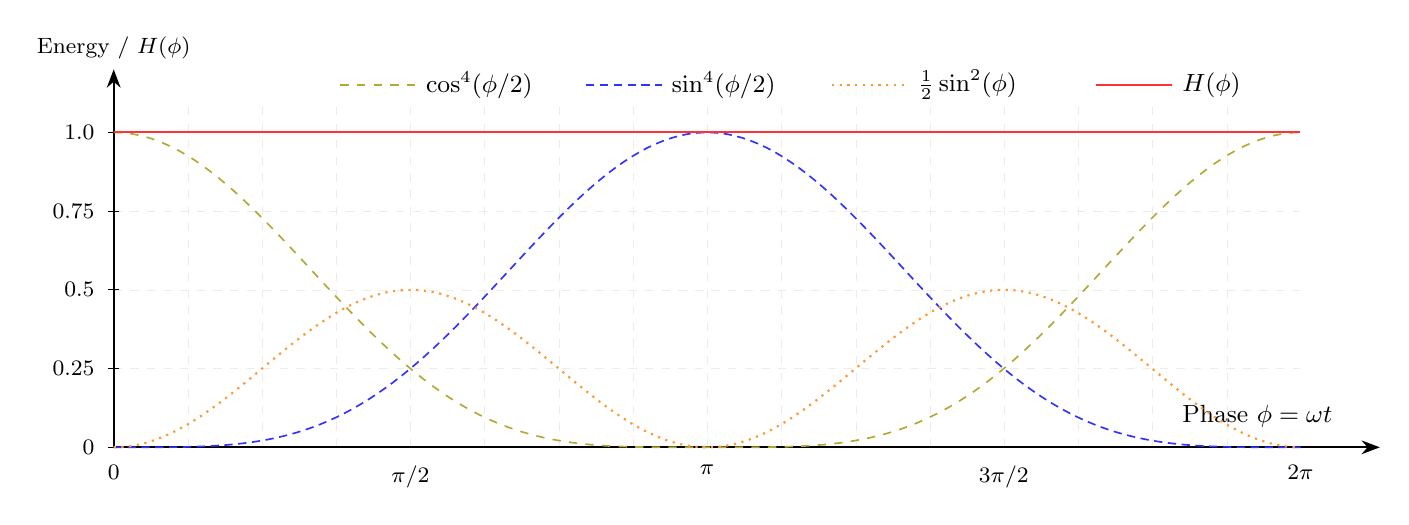
\begin{tikzpicture}[
    % Width unchanged; y unit length extended (2.5cm -> 4.0cm) to increase vertical height
    x=2.4cm, 
    y=4.0cm, 
    >=Stealth
]
    % --- Grid ---
    \draw[gray!15, xstep=0.3927, ystep=0.25, dashed, very thin] (0,0) grid (6.28, 1.1);
    
    % --- Coordinate axes ---
    \draw[thick, ->] (0,0) -- (6.7,0); % Horizontal axis
    \draw[thick, ->] (0,0) -- (0,1.2) node[above, font=\footnotesize] {Energy / $H(\phi)$};

    % --- Axis label (positioned independently for flexible adjustment) ---
    % Adjust the (x, y) values to move the label upward or leftward as needed.
    % Currently placed slightly upper-left of the axis tip at (6.5, 0.1).
    \node[font=\small, anchor=east] at (6.5, 0.1) {Phase $\phi = \omega t$};

    % Font sizes in decreasing order: \small, \footnotesize, \scriptsize, \tiny
    % --- Tick marks and labels ---
    % Vertical axis
    \foreach \y in {0, 0.25, 0.5, 0.75, 1.0} {
        \draw (0.03, \y) -- (-0.03, \y);
        \node[left, font=\footnotesize] at (-0.05, \y) {\y};
    }
    % Horizontal axis
    \node[below, font=\footnotesize, yshift=-3pt] at (0, 0) {0};
    \node[below, font=\footnotesize, yshift=-3pt] at (1.57, 0) {$\pi/2$};
    \node[below, font=\footnotesize, yshift=-3pt] at (3.14, 0) {$\pi$};
    \node[below, font=\footnotesize, yshift=-3pt] at (4.71, 0) {$3\pi/2$};
    \node[below, font=\footnotesize, yshift=-3pt] at (6.28, 0) {$2\pi$};

    % --- Function plots ---
    \draw[olive!70, dashed, semithick, domain=0:6.28, samples=150] 
        plot (\x, {(cos(\x * 180 / 3.14 / 2)^4)});

    \draw[blue!80, densely dashed, semithick, domain=0:6.28, samples=150] 
        plot (\x, {(sin(\x * 180 / 3.14 / 2)^4)});

    \draw[orange!80, dotted, thick, domain=0:6.28, samples=150] 
        plot (\x, {0.5 * (sin(\x * 180 / 3.14)^2)});

    \draw[red!80, thick] (0, 1.0) -- (6.28, 1.0);

    % --- Legend ---
    \begin{scope}[shift={(1.2, 1.15)}]
        \draw[olive!70, dashed, semithick] (0,0) -- (0.4,0) node[right, font=\small, black] {$\cos^4(\phi/2)$};
        \draw[blue!80, densely dashed, semithick] (1.3,0) -- (1.7,0) node[right, font=\small, black] {$\sin^4(\phi/2)$};
        \draw[orange!80, dotted, thick] (2.6,0) -- (3.0,0) node[right, font=\small, black] {$\frac{1}{2}\sin^2(\phi)$};
        \draw[red!80, thick] (4.0,0) -- (4.4,0) node[right, font=\small, black] {$H(\phi)$};
    \end{scope}

\end{tikzpicture}%
    }
    \caption{\justifying \textbf{Energy conservation and internal dynamics in the 0-Sphere electron model.} The graph demonstrates the temporal evolution of energy components during internal circulation between thermal kernels. The blue dashed line represents the thermal potential energy (TPE) of kernel~$A$ following $\cos^4(\phi/2)$, the orange dotted line shows kernel~$B$'s TPE as $\sin^4(\phi/2)$, and the green dashed line depicts the photon sphere kinetic energy $(1/2)\sin^2(\phi)$ with characteristic double-frequency oscillation. The red solid line $H(\phi)$ represents the total energy, remaining constant throughout all phases, confirming perfect energy conservation as required by Eq. ~\eqref{eq:energy_conservation}. The quartic temperature dependence follows from black-body radiation principles, while the sinusoidal kinetic energy profile provides the physical foundation for the $\sin\theta$-modulated internal motion used in the main text.
    }
    \label{fig:energy_conservation}
\end{figure*}

% ----------------------------------------
% Subsection H.1: Energy Conservation in the Dual-Kernel System
% ----------------------------------------
\subsection{Energy Conservation in the Dual-Kernel System}
\label{subsec:energy_conservation}

The fundamental starting point for the internal dynamics of the 0-Sphere electron model lies in the energy conservation law governing energy circulation between two internal kernels, designated as kernel~$A$ and kernel~$B$. The electron’s rest energy oscillates between these kernels through a mediating photon sphere that temporarily carries kinetic energy during the transfer process~\cite{hanamura16759284}.

The complete energy conservation relation takes the form
\begin{equation}
\boxed{E_0
= E_0\!\left[
\cos^4\!\left(\frac{\omega t}{2}\right)
+ \sin^4\!\left(\frac{\omega t}{2}\right)
+ \frac{1}{2}\sin^2(\omega t)
\right]},
\label{eq:energy_conservation}
\end{equation}
where $E_0$ denotes the total rest energy of the electron and $\omega$ is the fundamental oscillation frequency of the internal energy exchange. The first two terms represent the thermal potential energies stored in kernels~$A$ and~$B$, respectively, while the third term corresponds to the kinetic energy of the photon sphere during energy transfer.

Equation~\eqref{eq:energy_conservation} demonstrates that the electron maintains exact energy conservation throughout all temporal phases of the internal cycle. The quartic dependence $\cos^4(\omega t/2)$ and $\sin^4(\omega t/2)$ arises from the requirement that each kernel behaves as an effective black-body radiator, consistent with the Stefan--Boltzmann law, where radiative intensity scales with the fourth power of temperature~\cite{hanamura17765097}.

The mathematical structure of this identity reveals three distinct oscillatory components operating at different effective frequencies. The thermal potential energies of the kernels oscillate with half the fundamental frequency, producing the characteristic $720^\circ$ periodicity associated with spin-$\tfrac{1}{2}$ systems. In contrast, the photon-sphere kinetic energy oscillates at the full frequency $\omega$, providing the dynamical mechanism that enables continuous energy circulation between the kernels.

The complementary behavior of these energy components, together with their exact conservation, is illustrated in Fig.~\ref{fig:energy_conservation}. This structure forms the dynamical substrate from which the sinusoidal internal motion derived in the next sections naturally emerges.


% ----------------------------------------
% Subsection H.2: Reinterpretation of Positive and Negative Energy States
% ----------------------------------------
\subsection{Reinterpretation of Positive and Negative Energy States}
\label{subsec:reinterpretation_positive}

The reinterpretation of Zitterbewegung as a real physical oscillation, rather than a purely mathematical artifact of the Dirac equation, provides an essential conceptual foundation for the present framework. In earlier work~\cite{hanamura17760132}, we proposed that the positive- and negative-energy solutions of the Dirac equation should be understood as thermal potential energy states associated with internal components of a composite electron model.

In conventional quantum field theory, negative-energy solutions are typically addressed through the Dirac sea or particle--antiparticle creation formalisms. However, such interpretations obscure the physical origin of the characteristic oscillatory behavior known as Zitterbewegung. By contrast, treating the electron as a thermodynamically active system composed of internal energy reservoirs allows this oscillation to be understood as a real process of energy emission and absorption.

Within this reinterpretation, the wave functions corresponding to \textbf{positive and negative energy states describe alternating phases of thermal radiation and absorption between internal kernels.} It is worth emphasizing that such a reinterpretation is difficult to accommodate within the conventional particle--antiparticle framework.

In standard interpretations, Zitterbewegung arises from interference between positive- and negative-energy solutions, yet the picture of a particle continuously oscillating against its antiparticle counterpart lacks a clear physical realization.
In particular, the question of how such oscillations persist without spatial separation of particle and antiparticle remains conceptually obscure.

\textbf{The present model does not reject the antiparticle interpretation of negative-energy solutions.}
Rather, it proposes a complementary physical reading: negative energy is not treated as a static property at a given instant, but as a dynamical quantity associated with the temporal phase of thermal potential energy exchange.
At any fixed time slice, it is indeed difficult to assign a meaningful notion of negative mass.
However, when viewed through time differentiation, a thermal potential energy that decreases with phase naturally behaves as an effective negative-energy contribution.

Within the 0-Sphere model, one internal kernel undergoes a phase during which its thermal potential energy is radiatively emitted, corresponding to a monotonic decrease of effective mass with respect to the internal time parameter.
Simultaneously, the conjugate kernel absorbs the radiated energy, exhibiting a complementary increase in effective mass.
This paired evolution provides a concrete physical realization of the positive- and negative-energy structure of the Dirac equation.

Because both thermal potential energies coexist within a single electron as an inseparable pair, Zitterbewegung emerges as a continuously existing internal oscillation rather than a transient interference phenomenon.
In this way, the dual-kernel structure furnishes a natural and physically intuitive substrate for the persistent Zitterbewegung implied by relativistic quantum mechanics.

This perspective entails a crucial conceptual shift: the positive- and negative-energy solutions of the Dirac equation are interpreted \textbf{not as static states, but as dynamical processes} evolving along an internal time parameter.
When read in this manner, the distinction between positive and negative energy does not correspond to an instantaneous property of the electron, but to the direction of energy flow within a phase-dependent circulation.

Such a \textbf{process-based interpretation} naturally invites a formulation in terms of temporal differentiation and accumulation.
Local changes in thermal potential energy are described at the level of time derivatives, while the physically observable effects of Zitterbewegung arise from their accumulation over a complete internal cycle.
This passage from differential description to integral characterization provides the conceptual basis for treating the internal dynamics through line integrals along admissible paths.

The resulting \textbf{differential--integral correspondence} mirrors well-known structures in classical field theory, such as the equivalence between the differential and integral forms of Maxwell's equations.
In the present context, it is precisely this correspondence that enables the emergence of geometric phase from internal energy circulation, thereby linking relativistic quantum structure to thermodynamic and topological foundations.

The characteristic Zitterbewegung frequency, approximately $2mc^2/\hbar$, then reflects the intrinsic timescale of internal energy circulation rather than interference between abstract frequency components. This viewpoint transforms Zitterbewegung from a formal curiosity into a direct manifestation of internal thermodynamic dynamics.

This reinterpretation provides the conceptual bridge between relativistic quantum mechanics and the internal energy circulation described by the 0-Sphere model. In particular, it justifies treating the dual-kernel system and its associated photon sphere as physically real structures, whose dynamics give rise to the sinusoidal internal motion derived below.


% ----------------------------------------
% Subsection H.3: Derivation of the Sinusoidal State Function from Temperature Gradients
% ----------------------------------------
\subsection{Derivation of the Sinusoidal State Function from Temperature Gradients}
\label{subsec:sinusoidal_derivation}

This derivation provides the thermodynamic foundation for the $\sin\theta$-modulated internal motion illustrated in Fig.~\ref{fig:embedding}, where the phase-dependent displacement of the internal energy center emerges from temperature-gradient-driven energy circulation.

The emergence of the sinusoidal internal motion employed in the main text finds its physical origin in the temperature gradients generated by energy exchange between the two kernels. This derivation establishes that the $\sin\theta$ dependence is not an assumed functional form, but a direct consequence of thermodynamic energy circulation.

The thermal energies stored in the kernels are given by
\begin{align}
T_{e1} &= E_0 \cos^4\!\left(\frac{\omega t}{2}\right), \label{eq:kernel_A_energy}\\
T_{e2} &= E_0 \sin^4\!\left(\frac{\omega t}{2}\right), \label{eq:kernel_B_energy}
\end{align}
where $\theta = \omega t$ defines the internal phase parameter. Because the kernels remain fixed in space, while their energies vary in time, the relevant gradients are temporal rather than spatial.

Taking derivatives with respect to $\theta$, one obtains
\begin{align}
\mathrm{grad}\, T_{e1}
&= -2E_0 \cos^3\!\left(\frac{\theta}{2}\right)
      \sin\!\left(\frac{\theta}{2}\right), \label{eq:grad_Te1}\\
\mathrm{grad}\, T_{e2}
&=  2E_0 \cos\!\left(\frac{\theta}{2}\right)
      \sin^3\!\left(\frac{\theta}{2}\right). \label{eq:grad_Te2}
\end{align}

The net temperature gradient driving energy circulation between the kernels is therefore
\begin{align}
\mathrm{grad}(T_{e2}-T_{e1})
&= 2E_0 \cos\!\left(\frac{\theta}{2}\right)
       \sin\!\left(\frac{\theta}{2}\right) \notag\\
&= E_0 \sin\theta.
\label{eq:temperature_gradient}
\end{align}

Equation~\eqref{eq:temperature_gradient} demonstrates that the driving force associated with the internal temperature difference is intrinsically sinusoidal. This force induces simple harmonic motion of the photon sphere, providing the physical basis for the $\sin\theta$-modulated internal dynamics discussed in the main text.

The velocity of the photon sphere, which carries kinetic energy during the transfer process, is therefore governed by
\begin{equation}
\boxed{
u_{\gamma^*} = -E_0 \sin\theta,
}
\label{eq:photon_velocity}
\end{equation}
where the negative sign indicates energy flow from the higher-temperature kernel toward the lower-temperature kernel~\cite{hanamura16759284}.

This result establishes the central conclusion of the appendix: the sinusoidal internal motion arises inevitably from the thermodynamic structure of the dual-kernel system. The $\sin\theta$ dependence employed in the main text is thus not an arbitrary assumption, but the direct dynamical consequence of energy conservation and temperature-gradient-driven transport within the photon sphere.






\clearpage

\end{document}